\documentclass[9pt,serif,usenames,dvipsnames]{beamer}
\usetheme[progressbar=none]{metropolis}

\useoutertheme{metropolis}
\useinnertheme{metropolis}
\usefonttheme{metropolis}
\usecolortheme{beaver}

% ── Palette colori personalizzata (verde) ────────────────────────────
\definecolor{customgreen}{RGB}{0,128,0}
\definecolor{darkgray}{RGB}{64,64,64}
\definecolor{lightgray}{RGB}{128,128,128}
\definecolor{MSUgreen}{RGB}{0,192,0}

\setbeamercolor{structure}{fg=customgreen}
\setbeamercolor{frametitle}{fg=customgreen}
\setbeamercolor{title}{fg=customgreen}
\setbeamercolor{author}{fg=customgreen}
\setbeamercolor{date}{fg=customgreen}
\setbeamercolor{section in toc}{fg=customgreen}
\setbeamercolor{subsection in toc}{fg=customgreen}
\setbeamercolor{item}{fg=customgreen}
\setbeamercolor{subitem}{fg=customgreen}
\setbeamercolor{subsubitem}{fg=customgreen}
\setbeamercolor{section in head/foot}{fg=customgreen}
\setbeamercolor{subsection in head/foot}{fg=customgreen}
\setbeamercolor{titlelike}{fg=customgreen}
\setbeamercolor{section title}{fg=customgreen}
\setbeamercolor{section name}{fg=customgreen}
\setbeamercolor{separation line}{fg=customgreen}
\setbeamercolor{fine separation line}{fg=customgreen}
\setbeamercolor{progress bar}{fg=customgreen,bg=customgreen!30}
\setbeamercolor{alerted text}{fg=customgreen}
\setbeamercolor{block title alerted}{bg=customgreen,fg=white}
\setbeamercolor{block body alerted}{bg=customgreen!10,fg=black}
\setbeamercolor{block title example}{bg=customgreen!70,fg=white}
\setbeamercolor{block body example}{bg=customgreen!5,fg=black}
\setbeamercolor{block body}{bg=mDarkTeal!5}
\setbeamercolor{block title}{bg=mDarkTeal,fg=black!2}

\setbeamertemplate{footline}[frame number]
\setbeamertemplate{page number in head/foot}[totalframenumber]
\setbeamercolor{background canvas}{bg=white}
\setbeamercovered{transparent=15}
\setbeamersize{text margin left=5mm,text margin right=5mm}
\setbeamertemplate{theorems}[ams style]
\setbeamertemplate{navigation symbols}{}
\setbeamertemplate{frametitle}[default][center]

% ── Pacchetti ─────────────────────────────────────────────────────────────────
\usepackage{amsmath,amssymb}
\usepackage[many]{tcolorbox}
\usepackage{multirow,adjustbox,array}
\usepackage{tikz}
\usepackage{xcolor,xspace}
\usepackage{booktabs}
\usepackage[table]{xcolor}
\usepackage{colortbl}
\usepackage{graphicx}
\usepackage{qrcode}
\usetikzlibrary{arrows,shapes,decorations.pathreplacing,arrows.meta,positioning}

% ── Comandi tabella ───────────────────────────────────────────────────────────
\newcommand\Tstrut{\rule{0pt}{2.9ex}}
\newcommand\Bstrut{\rule[-1.2ex]{0pt}{0pt}}
\newcolumntype{x}[1]{>{\centering\let\newline\\\arraybackslash\hspace{0pt}}p{#1}}

\definecolor{placebg}{HTML}{E1F5EE}
\definecolor{placetxt}{HTML}{085041}
\definecolor{placeacc}{HTML}{1D9E75}
\definecolor{attackbg}{HTML}{E6F1FB}
\definecolor{attacktxt}{HTML}{0C447C}
\definecolor{attackacc}{HTML}{378ADD}
\definecolor{fortifybg}{HTML}{FAEEDA}
\definecolor{fortifytxt}{HTML}{633806}
\definecolor{fortifyacc}{HTML}{BA7517}
\definecolor{ellipsisbg}{HTML}{F5F5F3}
\definecolor{ellipsistxt}{HTML}{888780}

\newcolumntype{C}[1]{>{\centering\arraybackslash}p{#1}}

% ── Pseudocodice semplice ─────────────────────────────────────────────────────
\newenvironment{pseudocode}{%
	\begin{tabbing}%
		\hspace{1.4em}\=\hspace{1.4em}\=\hspace{1.4em}\=\kill%
	}{%
	\end{tabbing}%
}
\newcommand{\pckw}[1]{\textbf{#1}}
\newcommand{\pccmt}[1]{\textcolor{gray}{\small\textit{// #1}}}

% ── Titolo ────────────────────────────────────────────────────────────────────
\title[]{%
	{\color{darkgray}\rmfamily\itshape\textbf{TensorFlowers}}%
}

\author[]{%
	{\color{darkgray}\textsc{\textbf{Autore}}} \hfill
	\url{autore@unife.it}%
}

\titlegraphic{%
	\begin{tikzpicture}[overlay, remember picture]
		\node[at=(current page.south east), anchor=south east,
		xshift=-0.5cm, yshift=0.5cm]{%
			%\includegraphics[width=.18\textwidth]{unife.png}%
		};
	\end{tikzpicture}%
}

\institute[]{%
	Alice Zalambani, Davide Caravita, Giacomo Pampalone, Lorenzo Negrini, Marco Perrotta.
}

\date[2026]{{\color{darkgray}2026}}
\subject{Computer Science}

% =============================================================================
\begin{document}

	% ── Copertina ────────────────────────────────────────────────────────────────
	\begin{frame}[plain, noframenumbering]

		\begin{center}
			\vspace{0.8cm}

			{\usebeamerfont{title}
				\color{customgreen}
				\LARGE\textbf{TensorFlowers}\\[0.2cm]
			}

			\vspace{0.8cm}

			\color{customgreen}\rule{0.6\textwidth}{0.5pt}

			\vspace{1cm}

			{\color{darkgray}\large
				\textsc{Alice Zalambani},
				\textsc{Davide Caravita},
				\textsc{Giacomo Pampalone},\\
				\textsc{Lorenzo Negrini},
				\textsc{Marco Perrotta}
			}

			\vspace{0.9cm}
			\vspace{1.2cm}

			{\color{darkgray}\normalsize
				Department of Mathematics and Computer Science\\
				University of Ferrara
			}

			\vfill

			{\color{lightgray}2026}

		\end{center}

		\begin{tikzpicture}[overlay, remember picture]
			\node[at=(current page.south east), anchor=south east,
			xshift=-0.5cm, yshift=0.5cm]{%
				%\includegraphics[width=.14\textwidth]{unife.png}%
			};
		\end{tikzpicture}

	\end{frame}

	% ── Indice ────────────────────────────────────────────────────────────────────
	\begin{frame}
		\frametitle{Outline}
		\setbeamertemplate{itemize item}[ball]
		\setbeamercolor{itemize item}{fg=structure}
		\begin{center}
			\large
			\begin{itemize}
				\setlength{\itemsep}{0.6em}
				\item<1-> Introduzione \& Obiettivo
				\item<2-> Analisi del Dataset 
				\item<3-> Approccio Scelto 
				\item<4-> Altri Approcci
				\item<5-> Esperimenti \& Risultati
				\item<6-> Conclusioni
			\end{itemize}
		\end{center}
	\end{frame}

	% =============================================================================
	\section{Introduzione \& Obiettivo}

	\begin{frame}{\centering Introduzione \& Obiettivo}
		\textbf{Obiettivi:}
		\begin{itemize}
			\item Studio del problema e delle soluzioni note nella letteratura.
			\item Progettazione di una rete neurale con l'obbiettivo di identificare/classificare 5 differenti classi di fiori.
		\end{itemize}
	\end{frame}

	% =============================================================================
	\section{Analisi del Dataset}

		\begin{frame}{\centering Dataset TF Flowers}
		\begin{columns}[T]
			
			% Colonna immagini
			\begin{column}{0.35\textwidth}
				\begin{center}
					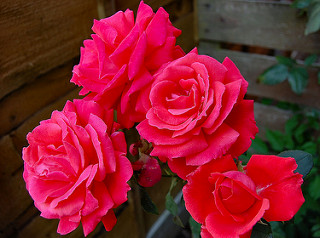
\includegraphics[width=0.8\linewidth]{fiore1.jpg}
					
					\vspace{0.15cm}
					
					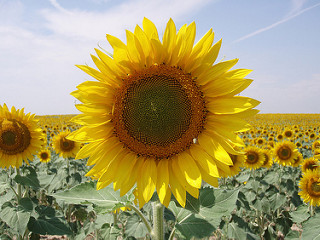
\includegraphics[width=0.8\linewidth]{fiore2.jpg}
					
					\vspace{0.15cm}
					
					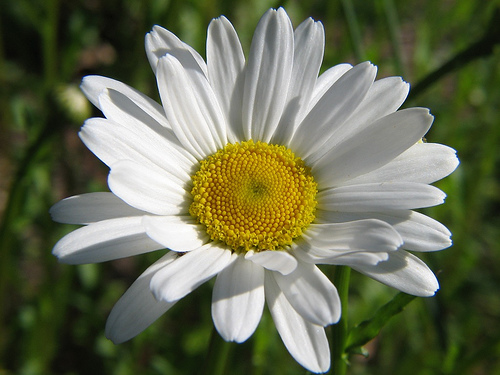
\includegraphics[width=0.8\linewidth]{fiore3.jpg}
				\end{center}
			\end{column}
			
			% Colonna descrizione
			\begin{column}{0.62\textwidth}
				\begin{block}{Caratteristiche principali}
					\begin{itemize}
						\item Numero immagini: \textbf{3670}
						\item Numero classi: \textbf{5}
						\item Formato: immagini RGB a dimensione variabile
						\item Task: classificazione di specie floreali
					\end{itemize}
				\end{block}
				
				\vspace{0.1cm}
				
				\begin{block}{Classi presenti}
				\begin{columns}
					\begin{column}{0.5\textwidth}
						\begin{itemize}
							\item Daisy
							\item Dandelion
							\item Roses
						\end{itemize}
					\end{column}
					\begin{column}{0.5\textwidth}
						\begin{itemize}
							\item Sunflowers
							\item Tulips
						\end{itemize}
					\end{column}
				\end{columns}
				\end{block}
				
				\vspace{0.05cm}
				
				\begin{alertblock}{Uso tipico del dataset}
					Addestrare un modello di \textbf{Image Classification}
					capace di riconoscere automaticamente la specie del fiore
					a partire dall'immagine in ingresso.
				\end{alertblock}
				
			\end{column}
			
		\end{columns}
	\end{frame}

	\begin{frame}{\centering Studio del Dataset}
		\begin{columns}[T]
			
			\begin{column}{0.40\textwidth}
				\begin{block}{Distribuzione delle classi}
					\begin{itemize}
						\item Totale immagini: 3.670
						\item Media per classe: $\sim$734 immagini
					\end{itemize}
				\end{block}
				
				\vspace{0.3cm}
				
				\begin{alertblock}{Osservazione}
					Le classi risultano \textbf{abbastanza bilanciate} 
					(range 630--900), riducendo il rischio di 
					bias nel training del modello.
				\end{alertblock}
			\end{column}

			\begin{column}{0.58\textwidth}
				\vspace{1.0 cm}
				\begin{center}
					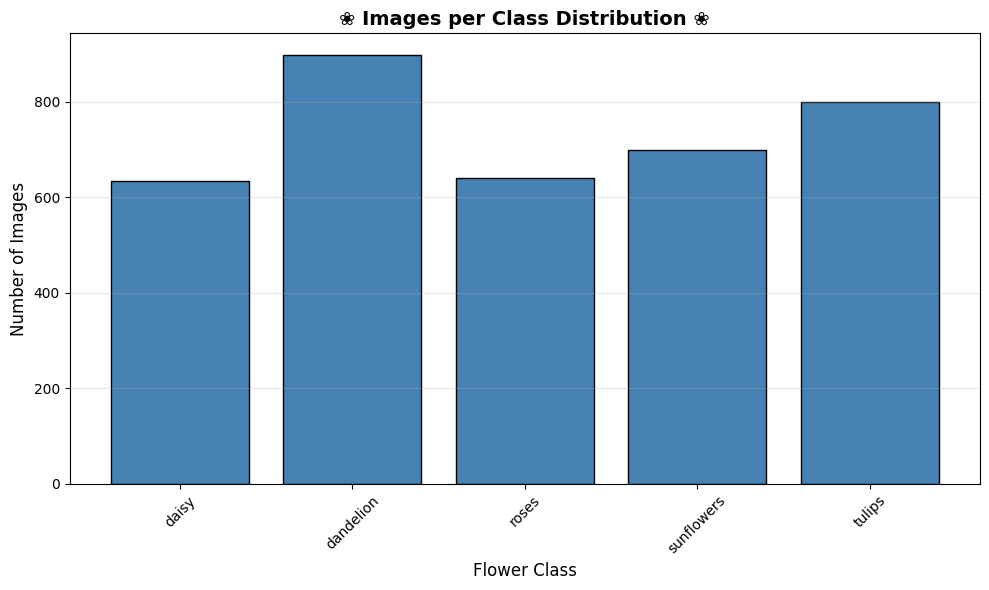
\includegraphics[width=0.95\linewidth]{plot.png}
				\end{center}
			\end{column}
			
		\end{columns}
	\end{frame}

	\begin{frame}{\centering Preprocessing e Split del Dataset}
    \begin{columns}[T]

        \begin{column}{0.42\textwidth}
            \begin{block}{Suddivisione del Dataset}
                \begin{itemize}
                    \item \textbf{Train:} 75\% delle immagini
                    \item \textbf{Validation:} 15\% delle immagini
                    \item \textbf{Test:} 10\% delle immagini
                \end{itemize}
            \end{block}

            \vspace{0.2cm}

            \begin{alertblock}{Scelta Progettuale}
                Tali immagini sono state \textbf{mantenute}: risultano
                bilanciate tra le classi e la rimozione avrebbe ridotto
                ulteriormente un dataset già limitato.
            \end{alertblock}
        \end{column}

        \begin{column}{0.55\textwidth}
            \begin{block}{Esempi di Immagini Difficoltose}
                Fiori parzialmente visibili, illuminazione sfavorevole
                o soggetti multipli e sfocati.
            \end{block}
            \vspace{0.15cm}
            \begin{center}
                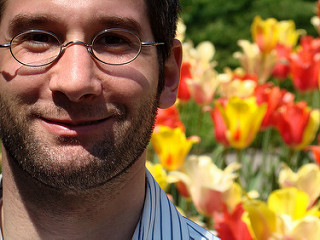
\includegraphics[width=0.45\linewidth]{diff1.jpg}\hspace{0.3cm}
                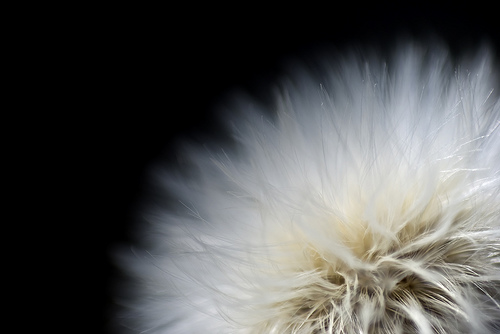
\includegraphics[width=0.45\linewidth]{diff2.jpg}\\[0.2cm]
                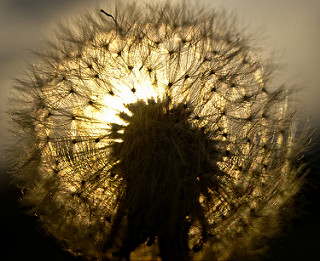
\includegraphics[width=0.45\linewidth]{diff3.jpg}
            \end{center}
        \end{column}

    \end{columns}
\end{frame}

	% =============================================================================
	\section{Approccio Scelto}

	\begin{frame}{\centering Architettura: Rete Convoluzionale (CNN)}

		\begin{columns}[T]
			\begin{column}{0.48\textwidth}
				\begin{block}{Utilizzo di CNN}
					\begin{itemize}
						\item Progettate per dati con \textbf{struttura spaziale}
						\item I primi layer apprendono \textbf{pattern locali}
						(bordi, texture, colori)
						\item I layer profondi \textbf{combinano} tali pattern
						in rappresentazioni semantiche
					\end{itemize}
				\end{block}

				\vspace{0.15cm}

				\begin{block}{Architetture di Riferimento}
					\begin{itemize}
						\item \textbf{ResNet}: batch norm post-attivazione
						\item \textbf{VGGNet}: kernel piccoli e layer
						multipli in sequenza
					\end{itemize}
				\end{block}

			\end{column}

			\begin{column}{0.48\textwidth}
				\begin{center}
					\textbf{ResNet}\\[0.1cm]
					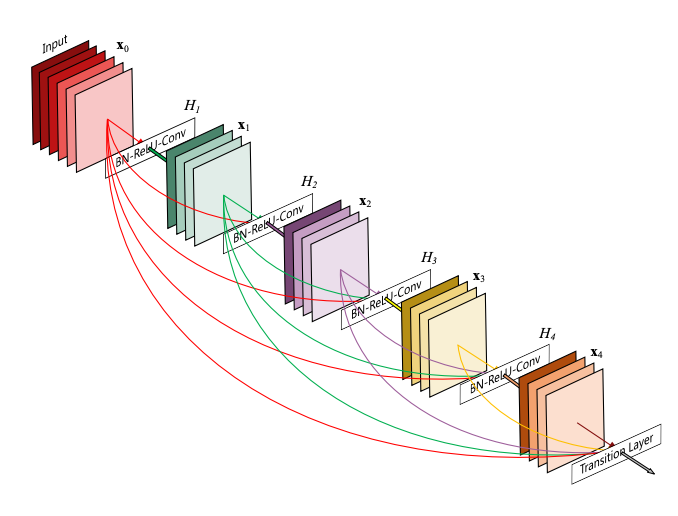
\includegraphics[width=0.80\linewidth]{resnet.png}\\[0.2cm]
					\textbf{VGGNet}\\[0.1cm]
					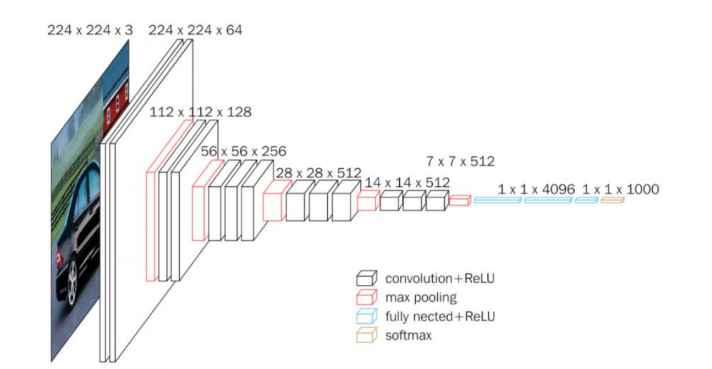
\includegraphics[width=0.80\linewidth]{vggnet.png}
				\end{center}
			\end{column}
		\end{columns}

	\end{frame}

	\begin{frame}{\centering Struttura della Rete, Schema Generale}
		\begin{columns}[T]

			\begin{column}{0.48\textwidth}
				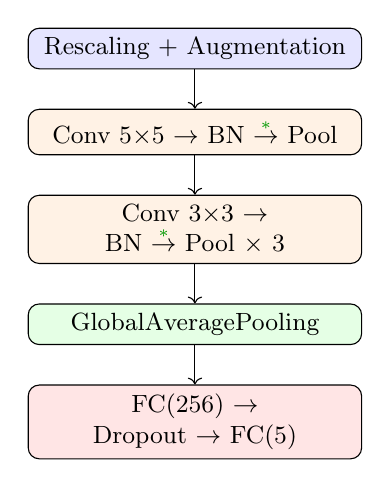
\begin{tikzpicture}[node distance=0.5cm, every node/.style={font=\small}]
					\node (pre) [draw, rounded corners, fill=blue!10, text width=4cm, align=center] 
						{Rescaling + Augmentation};
					\node (conv1) [draw, rounded corners, fill=orange!10, text width=4cm, align=center, below=of pre] 
						{Conv 5$\times$5 $\to$ BN $\overset{\textcolor{green!60!black}{*}}{\to}$ Pool};
					\node (conv2) [draw, rounded corners, fill=orange!10, text width=4cm, align=center, below=of conv1] 
						{Conv 3$\times$3 $\to$ BN $\overset{\textcolor{green!60!black}{*}}{\to}$ Pool $\times$ 3};
					\node (gap) [draw, rounded corners, fill=green!10, text width=4cm, align=center, below=of conv2] 
						{GlobalAveragePooling};
					\node (fc) [draw, rounded corners, fill=red!10, text width=4cm, align=center, below=of gap] 
						{FC(256) $\to$ Dropout $\to$ FC(5)};

					\draw[->] (pre) -- (conv1);
					\draw[->] (conv1) -- (conv2);
					\draw[->] (conv2) -- (gap);
					\draw[->] (gap) -- (fc);
				\end{tikzpicture}
			\end{column}

			\begin{column}{0.48\textwidth}
				\begin{alertblock}{Scelta Progettuale}
					Il \textbf{secondo layer Conv 3$\times$3} presente in
					ogni blocco è stato \textbf{rimosso}: sperimentalmente
					facendo questo si ottengono risultati migliori, evitando overfitting
					su un dataset di dimensioni limitate.
				\end{alertblock}
			\end{column}

		\end{columns}
	\end{frame}

	\begin{frame}{\centering Struttura della Rete, Preprocessing}
		\begin{block}{Preprocessing}
			\begin{itemize}
				\item \textbf{Rescaling}: valori da $[0, 255]$ a $[0, 1]$
				\item \textbf{Data Augmentation}: flip orizzontale,
				rotazione e zoom casuali
			\end{itemize}
		\end{block}
	\end{frame}

	\begin{frame}{\centering Struttura della Rete, Blocco Convoluzionale}
		\begin{block}{Blocco Convoluzionale $\times 4$}
			Ripetuto con 32 – 64 – 128 – 256 filtri:
			\begin{itemize}
				\item Conv2D \textbf{5$\times$5} (solo primo blocco),
				\textbf{3$\times$3} nei successivi + ReLU (''estrazione'' pattern dalle immagini che verrano usati come feture)
				\item Batch Normalization
				\item MaxPooling (per riduzione dimensinalita dell'immagine)
			\end{itemize}
		\end{block}

		\vspace{0.15cm}

		\begin{block}{Classificatore}
			\begin{itemize}
				\item \textbf{GlobalAveragePooling}: 256 feature map
				$\rightarrow$ vettore 256 (fai avg per ogni matrice per ottenere unico vettore)
				\item FC 256 $\rightarrow$ Dropout $\rightarrow$
				FC 5 (softmax) (classificazione dato vettore)
			\end{itemize}
		\end{block}
	\end{frame}
		

	% =============================================================================
\begin{frame}{\centering Bagging di Modelli \& Fine Tuning di ResNet-50}
    \begin{columns}[T]

        \begin{column}{0.48\textwidth}
            \begin{block}{Ensemble (Bagging)}
                Combinazione di 5 checkpoint del modello custom:
                \begin{itemize}
                    \item Ogni modello riceve lo stesso input
                    \item Le predizioni vengono \textbf{mediate}
                \end{itemize}
            \end{block}

            \vspace{0.05cm}

            \begin{block}{Fine Tuning ResNet-50}
                \begin{itemize}
                    \item Base: \textbf{ResNet-50} pretrained su ImageNet,
                    layer convoluzionali \textbf{frozen}
                    \item Head custom: \texttt{AvgPool(7$\times$7)}
                    $\to$ \texttt{Flatten} $\to$ \texttt{FC(256)}
                    $\to$ \texttt{Dropout(0.5)} $\to$ \texttt{FC(5)}
					\item Ottimizzatore: \textbf{Adam}
                    \item Training: \textbf{20 epoche}
                \end{itemize}
            \end{block}
        \end{column}

        \begin{column}{0.48\textwidth}
            \begin{block}{Schema Ensemble}
                \begin{center}
                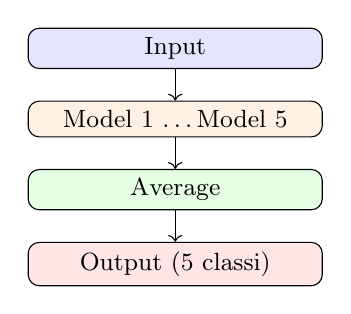
\begin{tikzpicture}[node distance=0.4cm, every node/.style={font=\small}]
                    \node (inp) [draw, rounded corners, fill=blue!10, text width=3.5cm, align=center]
                        {Input};
                    \node (m1) [draw, rounded corners, fill=orange!10, text width=3.5cm, align=center, below=of inp]
                        {Model 1 \dots Model 5};
                    \node (avg) [draw, rounded corners, fill=green!10, text width=3.5cm, align=center, below=of m1]
                        {Average};
                    \node (out) [draw, rounded corners, fill=red!10, text width=3.5cm, align=center, below=of avg]
                        {Output (5 classi)};
                    \draw[->] (inp) -- (m1);
                    \draw[->] (m1) -- (avg);
                    \draw[->] (avg) -- (out);
                \end{tikzpicture}
                \end{center}
            \end{block}

            \vspace{0.15cm}

            \begin{alertblock}{Motivazione}
                Il bagging riduce la varianza combinando modelli
                addestrati su run diverse. Il fine tuning sfrutta
                le feature di ResNet-50 già generalizzate su ImageNet.
            \end{alertblock}
        \end{column}

    \end{columns}
\end{frame}


% =============================================================================
\section{Esperimenti \& Risultati}

\begin{frame}{\centering Setup Sperimentale}
    \begin{block}{Configurazione del Training}
        \begin{itemize}
            \item \textbf{Ottimizzatore:} Adam ($lr = 10^{-3}$, decay a plateau)
            \item \textbf{Epoche:} 100 (con Early Stopping, patience = 10)
            \item \textbf{Batch size:} 32
            \item \textbf{Metrica:} Accuracy e Loss su validation set e test set
        \end{itemize}
    \end{block}

    \vspace{0.2cm}

    \begin{alertblock}{Valutazione}
        Ogni modello è valutato tramite \textbf{5-fold cross-validation}
        sul training set, con test finale sul 10\% tenuto separato.
    \end{alertblock}
\end{frame}

\begin{frame}{\centering Risultati: Confronto Modelli}

    \begin{adjustbox}{width=\textwidth}
        \small
        \renewcommand{\arraystretch}{1.25}
        \begin{tabular}{lcccc}
            \toprule
            \textbf{Modello} & \textbf{Val Acc (\%)} & \textbf{Test Acc (\%)}
            & \textbf{Parametri} & \textbf{Epoche}\\
            \midrule
            \textbf{CNN Custom}        & -- & -- & $\sim$-- & -- \\
            Bagging (5 checkpoint)   & -- & -- & $\sim$-- & -- \\
            ResNet-50 Fine Tuning & -- & -- & $\sim$-- & -- \\
            \bottomrule
        \end{tabular}
    \end{adjustbox}

    \vspace{0.2cm}

    \begin{flushleft}
        \tiny Dati preliminari su split test 10\% (367 immagini).
        Accuracy media su 5-fold CV per i modelli custom.
    \end{flushleft}

    \begin{itemize}
        \item<1-> \textbf{Augmentation} porta un guadagno consistente
        (--\%) riducendo l'overfitting.
        \item<2-> \textbf{ResNet-50} sfrutta feature pre-apprese su
        ImageNet, dominando nettamente sul modello custom.
    \end{itemize}
\end{frame}
	% =============================================================================
\section{Conclusioni}

\begin{frame}{\centering Conclusioni}
    \onslide<1->{
        \begin{block}{Dataset bilanciato}
            TF Flowers risulta \alert{ben distribuito} tra le 5 classi,
            con le principali difficoltà legate a variabilità di
            illuminazione e occlusioni parziali.
        \end{block}
    }
    \vspace{0.15cm}
    \onslide<2->{
        \begin{block}{CNN Custom}
            La rete progettata da zero, con data augmentation e
            bagging, raggiunge circa \alert{--\% di accuracy},
            mostrando buona generalizzazione per un dataset limitato.
        \end{block}
    }
    \vspace{0.15cm}
    \onslide<3->{
        \begin{block}{Fine Tuning ResNet-50}
            Il transfer learning su ResNet-50 raggiunge \alert{--\%}
            di test accuracy, confermando l'efficacia del riutilizzo
            di feature pre-addestrate su ImageNet.
        \end{block}
    }

\end{frame}


\begin{frame}
    \centering
    \vspace{1.5cm}
    {\Huge \textbf{Grazie per l'attenzione!}}
    
    \vspace{0.8cm}
    {\large Codice e progetto disponibili su GitHub}
    
    \vspace{1.2cm}
    \qrcode[height=1.8in]{https://github.com/Perro2110/TensorFlowers}
    
    \vspace{1cm}
\end{frame}



\end{document}